\chapter{Aplicaci\'on Rna Folding Free Energy}\label{RNAFFE_chapter}
% (completar poniendo un ejemplo del archivo de salida)
\section{Motivaci\'on}
En la actualidad, los tratamientos para personas infectadas con HIV consisten de una intensiva terapia antirretroviral. Esta terapia puede ser vista como
una sucesi\'on de aplicaciones de antirretrovirales en el tiempo, donde en cada paso de la sucesi\'on se le suministra al paciente una combinaci\'on
de uno o m\'as antirretrovirales.

Cuando a una persona se le aplica un antirretroviral, el virus comienza a mutar hasta que logra hacerse resistente. \'Esto implica que el antirretroviral
deje de cumplir sus funciones principales y se deba buscar uno nuevo para continuar con el tratamieinto. El orden en que se aplican los antirretrovirales
y c\'omo \'estos son combinados, son factores muy importantes que determinan, entre otras cosas, el tiempo que transcurrir\'a hasta el momento en que el
virus sea resistente a todos los antirretrovirales. 

Hasta el momento, el impacto del escape a los antirretrovirales sobre la estructura secundaria no ha sido estudiada. Esta herramienta pretende recopilar
informaci\'on sobre como var\'ia la Energ\'ia Libre en la estructura secundaria del RNA viral a medida que los antirretrovirales son aplicados sobre
la persona infectada.

\newpage
\section{Soluci\'on}
Para alcanzar el objetivo propuesto, la idea principal puede ser resumida en el siguiente pseudo-algoritmo:
\begin{enumerate}
 \item Tomar una secuencia en representaci\'on del virus y todos los antirretrovirales conocidos hasta el momento.
 \item De todos los antirretrovirales, seleccionar solo aquellos que realmente pueden ser aplicados a la secuencia (un antirretroviral es aplicable
       sobre una secuencia cuando esta \'ultima no presenta resistencia alguna al mismo). De no haber ninguno aplicable, saltar al paso 7.
 \item Generar combinaciones de hasta tres antirretrovirales, utilizando aquellos seleccionados en el paso anterior.
 \item Aplicar cada combinaci\'on de antirretrovirales a la secuencia y obtener todas las secuencias mutantes.
 \item Calcular la FE de cada mutaci\'on.
 \item Ejecutar este proceso para cada una de las mutaciones obtenidas, recibiendo ahora como entrada cada una de esas secuencias mutadas. 
       Luego, saltar al paso 8.
 \item Informar resultado.
 \item Terminar.
\end{enumerate}
Al realizar estos pasos se genera un \'arbol donde cada nodo contiene, entre otras cosas, la secuencia del virus y la energ\'ia libre
(\textbf{FE}) para dicha secuencia. Cabe destacar que una hoja se caracteriza por tener una secuencia a la que ning\'un antirretroviral puede ser aplicado.

Para lograr el objetivo de ver c\'omo el suministro de antirretrovirales afecta la estructura secundaria del RNA viral, basta con seguir los distintos
caminos del \'arbol y observar como var\'ia la FE a medida que avanza la terapia. En la siguiente secci\'on se explicar\'a m\'as detalladamente como
se implement\'o la soluci\'on.

%\begin{figure}[ht]
%\centering
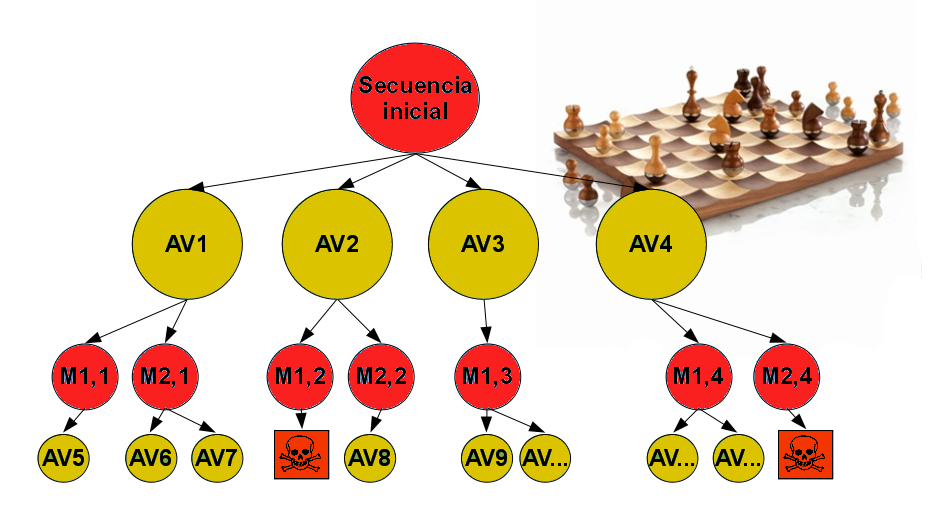
\includegraphics[width=\linewidth]{images/Arbol_ajedrez.png}
%\end{figure} 
En la imagen se muestra como se va generando el \'arbol, los c\'irculos de color rojo representan los nodos y los de color amarillo, los
antirretrovirales que se aplican para obtener la mutaci\'on del nodo hijo. Por otro lado, los recuadros que encierran una calavera establecen que la 
mutaci\'on obtenida es resistente a todos los antirretrovirales, por lo que esas ramas del \'arbol han llegado a su fin.

\section{Implementaci\'on}
En una visi\'on general, como se mencion\'o en otras oportunidades, la soluci\'on consta de armar un \'arbol y analizar los distintos caminos del mismo.
Debido a la gran cantidad de nodos que contiene este \'arbol, a lo costoso que es calcular la energ\'ia libre de una secuencia y a la necesidad de
contar con un motor combinatorio, se decidi\'o implementar la herramienta como la capa de aplicaci\'on del framework \fud. \'Esto nos brinda dos
facilidades imprescindibles:
\begin{enumerate}
 \item La posibilidad de poder realizar los c\'omputos de manera distribuida.
 \item Realizar, eficientemente, las combinaciones de antirretrovirales usando distintas pol\'iticas de combinaci\'on.
\end{enumerate}
  
Seg\'un lo mencionado en \ref{applicationLayer5}, la herramienta constituye el nivel m\'as alto del framework (la capa 5) y debe respetar la API
definida por la capa subyacente, es decir, la capa \textbf{L4-CombinatoryEngine}.
% (imagen de las ultimas dos capas l4, l5. resaltando cual es la interfaz y como se implemento)\\

\subsection{Datos de Entrada}
La herramienta recibe como entrada:
\begin{itemize}
  \item \textit{Secuencia Inicial del Virus}: Archivo que contiene una secuencia de nucle\'otidos representando el ADN del virus.
\begin{lstlisting}[basicstyle=\tt, frame=trBL, tabsize=4,fontadjust=true]
 CCTCAGGTCACTCTTTGGCAACGACCCCTCGTCACAATAAAGGTA
 GATAGGGGGGCAACTAAAGGAAGCTCTATTAGATACAGGAGACGG
 CAGATGATACAGTATTAGAAGAAATGAGTGATTTGCCAGGAA...
\end{lstlisting}
\vspace{.7cm}
 \item \textit{Conjunto de Antirretrovirales}: Archivo .xml conteniendo la base de datos de antirretrovirales.
\begin{lstlisting}[basicstyle=\tt, frame=trBL, tabsize=4,fontadjust=true]
<antivirals>
  ...
  
  <antiviral id="Didanosine" num ="1" type ="tRT" class ="cNRTI">	
    <resistance pos="164" aminos="R"/>
    <resistance pos="173" aminos="V"/>
  </antiviral>

  ...

</antivirals>
\end{lstlisting}

\end{itemize}

\subsection{Representaciones de Datos}
\subsubsection{Secuencia de nucle\'otidos}
Se representa a las secuencias de nucleótidos como cadenas de caracteres. Denotamos a las mismas se denotan como expresiones regulares.
\begin{itemize}
\item $nuc\_arn = a \vert u \vert c \vert g \vert \_$
\item $nuc\_adn = a \vert t \vert c \vert g \vert \_$
\end{itemize} 
Al igual que los nucle\'otidos, se representan los genes de ADN y ARN.
\begin{itemize}
\item $gen\_arn = (nuc\_arn)^{+}$
\item $gen\_adn = (nuc\_adn)^{+}$	
\end{itemize}

\subsubsection{Antirretrovirales}
Un Antirretroviral consta de, principalmente, un listado de posiciones de resistencia. Estas posiciones establecen en qu\'e mol\'eculas del virus
el antirretroviral se comporta de manera efectiva. En el dise\~no propuesto, estas posiciones no son s\'olo m\'s que un par $<pos , aminos>$ donde 
$pos \geq 0$ y $aminos$ es una lista de amino\'acidos. Es decir, la posici\'on de la resistencia describe un valor entero en el cual los amino\'acidos
act\'uan sobre el virus.
%\begin{figure}[h!]
  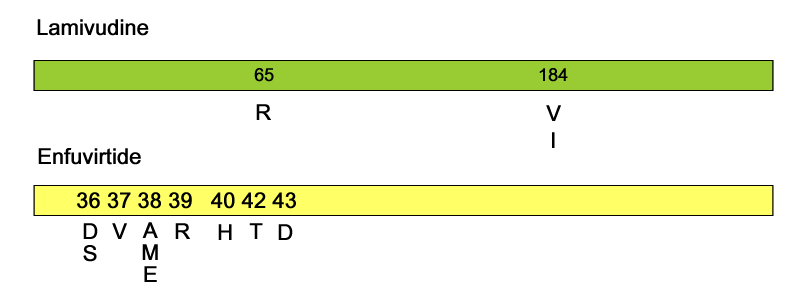
\includegraphics[scale=1]{images/Antivirals.png}\\
%  \caption{Ejemplo de dos antirretrovirales.} 
%\end{figure}

Adem\'as de este listado de posiciones, se incluye otro tipo de informaci\'on para el antirretroviral, como un identificador, un nombre, una clase y
un tipo.

\subsection{Predicci\'on de la Estructura Secundaria}
Esta predicci\'on consiste en obtener la \emph{estructura secundaria} a partir de la estructura primaria (ver \ref{estructuraSecundariaARN}). Existen
dos tipos de algoritmos para realizar esta tarea:
\begin{itemize}
 \item \textbf{Predicci\'on por \emph{minimal free energy (mfe)}}: Propuesto e implementado por Michael Zuker en el a\~no 1981 \cite{Zuker84}, utiliza programaci\'on
   din\'amica para encontrar la estructura secundaria que minimiza la energ\'ia libre.
 \item \textbf{Predicci\'on comparativa}: Utiliza diferentes m\'etodos para comparar secuencias y estructuras con el fin de obtener una estructura por ``consenso''\cite{Gardner04}.
\end{itemize}

Si bien la \textit{predicci\'on comparativa} presenta un incremento en la fidelidad de los resultados obtenidos con respecto a la \textit{predicci\'on
por mfe}, el primer tipo de predicci\'on requiere la existencia de un conjunto de secuencias relacionadas entre s\'i (hom\'ologas) y \'esto no siempre
es posible. En particular, en este trabajo s\'olo interesa poder realizar predicciones de la estructura secundaria a partir de una sola secuencia, por
lo que la predicci\'on comparativa fue descartada.

Entre las implementaciones de la predicci\'on por mfe, se destacan \textbf{RNAfold}\cite{Hofacker94} y \textbf{Mfold}. Ambas implementan el algoritmo propuesto por Michael
Zuker con complejidad $\mathcal{O}(N^{3})$ donde $N$ es la longitud de la secuencia.
A continuaci\'on se puede ver un ejemplo de una predicci\'on realizada con \textbf{RNAfold}.

\begin{verbatim}
combeng@fudepan:~$ RNAfold

  Input string (upper or lower case); 
  ....,....1....,....2....,....3....,....4...
  AAAGGCAACGGCCAU
  length = 15
  AAAGGCAACGGCCAU
  ...(((....)))..
  minimum free energy =  -4.40 kcal/mol
\end{verbatim}

El resultado obtenido es, precisamente, la energ\'ia libre y la estructura secundaria representada con par\'entesis y puntos. Donde los pares de
par\'entesis indican las bases ``apareadas'' o ``unidas'' y los puntos, las bases libres. Para este trabajo, solo es relevante la energ\'ia libre.

\subsection{Selecci\'on de los Antirretrovirales a Aplicar}
  Como se muestra en la siguiente secci\'on, cada nodo del \'arbol de ejecuci\'on dispone de una secuencia de nucle\'otidos. Para saber qu\'e 
  antirretrovirales combinar y as\'i avanzar en la terapia, es necesario obtener de la base de datos de antirretrovirales s\'olo aquellos a los que
  la secuencia del nodo no es resistente. Adem\'as de la condici\'on anterior, se seleccionan, preferentemente, aquellos que representen m\'as
  obst\'aculos para el virus, logrando que al mismo le sea m\'as costoso volverse resistente.\footnote{Para una explicaci\'on m\'as detallada,
  examinar el cap\'itulo 6 de ASO (\url{http://aso.googlecode.com})}
\newpage
\subsection{Preferencia en Combinaci\'on de Antirretrovirales}
Los antirretrovirales individualmente no suprimen la infecci\'on por VIH a largo plazo, por lo cual, actualmente se usan combinaciones de \'estos.
Las combinaciones de antirretrovirales act\'uan incrementando el n\'umero de obst\'aculos para la mutaci\'on viral, manteniendo bajo el n\'umero de
copias virales. En la figura \ref{antivirals_fsm} se muestra una M\'aquina de Estados Finita, de ahora en adelante FSM (por su acr\'onimo en
ingl\'es), representando c\'omo los antirretrovirales son combinados de acuerdo a la disponibilidad de los mismos. Como se explic\'o anteriormente, 
hay tres tipos de antirretrovirales (\textbf{NRTI}, \textbf{NNRTI}, \textbf{PI}). Dependiendo de la cantidad de cada uno que pueden ser aplicados a
la secuencia del nodo corriente, se escoge una pol\'itica de combinaci\'on seg\'un se detalla en la figura.

\begin{figure}[ht]
  \centering
  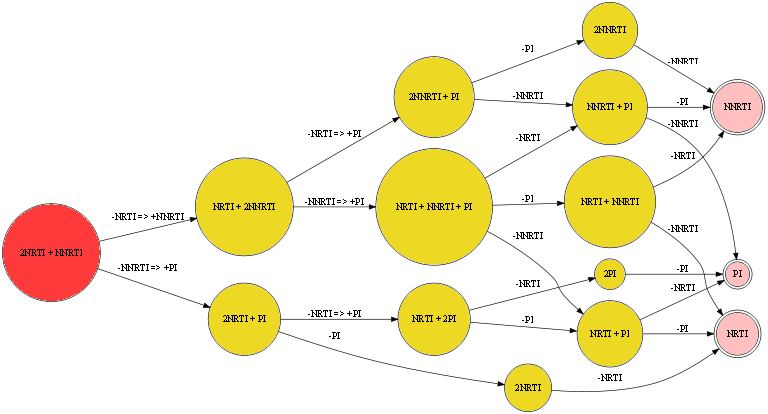
\includegraphics[width=\linewidth]{images/Antivirals_fsm.png}
  \label{antivirals_fsm}
\end{figure}

A modo de ejemplo supongamos que:
\begin{itemize}
 \item  El nodo ra\'iz del \'arbol contiene la secuencia inicial del virus, ll\'amese \textbf{X}.
 \item  Hay m\'as de dos antirretrovirales de cada tipo que se pueden aplicar a la secuencia \textbf{X}.
 \item  La pol\'itica de combinaci\'on del nodo ra\'iz es la representada por el primer estado de la FSM, \textbf{2NRTI+1NNRTI}.
\end{itemize}
Para este caso, la herramienta generar\'a todas las combinaciones de tres antirretrovirales, conteniendo dos del tipo \textbf{NRTI} y uno del tipo
\textbf{NNRTI}. Luego, por cada mutaci\'on obtenida al aplicar una combinaci\'on, se genera un hijo y se le ordena que se ejecute con la misma 
pol\'itica de combinaci\'on. En el momento en que el hijo debe ser ejecutado pueden ocurrir dos cosas:
\begin{enumerate}
 \item La cantidad de antirretrovirales de cada tipo que se le pueden aplicar a la mutaci\'on es suficiente para aplicar la misma pol\'itica de
   combinaci\'on del nodo padre.
 \item La cantidad de antirretrovirales de cada tipo que se le pueden aplicar a la mutaci\'on no es suficiente para aplicar la pol\'itica de 
   combinaci\'on del padre. En este caso, dependiendo del tipo del antirretroviral cuya cantidad es insuficiente, se cambia la pol\'itica de
   combinaci\'on para ejecutar el nodo. Estos cambios se realizan acorde a la FSM mostrada.
\end{enumerate}
%COMPLETAR: ACA TENDRIA QUE PONER XQ DANIEL HIZO ESA FSM.. PORQUE CONVIENE ELEGIR LOS ANTIVIRALES DE ESA FORMA

\subsection{Generaci\'on de Mutaciones a Partir de un Conjunto de Antirretrovirales}
Un antirretroviral esta compuesto, entre otras cosas, por un conjunto de resistencias. Suponga que, a modo de ejemplo, se toma el antirretroviral
Abacavir, el cual tiene como una de sus resistencias el amino\'acido \textbf{R} en la posici\'on \textbf{65}.

\begin{figure}[H]
  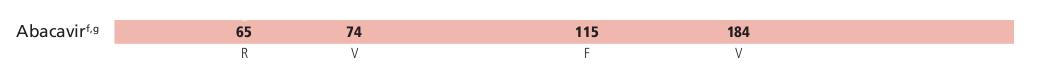
\includegraphics[width=\linewidth]{images/abacadir.png}
\end{figure}

Luego, si el triplete n\'umero \textbf{65} de la secuencia codifica el amino\'acido \textbf{R}, significa que dicha secuencia es resistente a tal antiviral.

\begin{figure}[H]
  
\includegraphics[width=\linewidth]{images/secuencia.png}
\end{figure}
En este caso, el triplete \textbf{ATT} codifica el amino\'acido \textbf{R}, lo cual hace a la mutaci\'on resistente al antirretroviral Abacavir.\\
Para lo obtenci\'on de las mutaciones a partir de un conjunto de antirretrovirales, se desarroll\'o un algoritmo que puede ser resumido en los siguientes pasos:
\newpage
\begin{enumerate}
  \item  Obtener el producto cartesiano de las resistencias de cada antirretroviral. Suponga el siguiente ejemplo,

    \textbf{Antirretrovirales}:
    \vspace{-.5cm}
    \begin{center}
      \emph {A = \{(1,G), (2,T)\}}
    
      \emph {B = \{(3,G), (2,T), (4,R)\}}
     \end{center}
      \scriptsize{En un par \emph{(X, Y)}: \emph{X} representa la posici\'on de la resistencia e \emph{Y} el amino\'acido al cual es resistente.}

      \normalsize{}Luego, el producto cartesiano entre \emph{A} y \emph{B} es:

  \emph{A} x \emph{B =} \vspace{-1cm}
                       \begin{center}
                          \emph{\{\{(1,G), (3,G)\}, \{(1,G), (2,T)\}, \{(1,G), (4,R)\}, \\
                          \{(2,T), (3,G)\}, \{(2,T), (2,T)\}, \{(2,T), (4,R)\}\}}
                       \end{center}
  \item  Aplicar las siguientes reglas a cada subconjunto \emph {S} del producto cartesiano:
      \begin{enumerate}
       \item Si $\exists(x,y),(z,w)\in\emph{S}$ : $x=z$  $\wedge$  $y\neq w$  $\mapsto$  Eliminar \emph{S} del producto cartesiano
         \footnote{Esto se debe a que no existen secuencias en las que para una posici\'on haya dos amino\'acidos.}.

       \item Si $\exists(x,y),(z,w)\in\emph{S}$ : $x=z$  $\wedge$  $y=w$  $\mapsto$  Eliminar una de las repeticiones de \emph{S}.
      \end{enumerate}
     	Una vez aplicadas las reglas, el producto cartesiano del paso anterior queda reducido a:
      
      \emph {A} x \emph{B' =} \vspace{-1cm}
      \begin{center}
         \emph{\{\{(1,G), (3,G)\}, \{(1,G), (2,T)\}, \{(1,G), (4,R)\}, \\
                \{(2,T), (3,G)\}, \{(2,T)\}, \{(2,T), (4,R)\}\}}
         \footnote{S\'olo se aplic\'o la regla del inciso b).}
      \end{center}

    \item  A partir del conjunto obtenido en el paso anterior (\emph{A} x \emph{B'}), se crea un nuevo conjunto (\emph{T}) conteniendo aquellos 
      subconjuntos de \emph{A} x \emph{B'} que tengan la menor cantidad de elementos.

   Es decir, 
   \begin{center}
     Sea \emph{S$_{1}$...S$_{n}$} $\in$ A x B' : \emph{S}$_{i}\in$ T \textbf{Sii} $\forall$\emph{S}$_{j}\in$S : \emph{count}(S$_{i}$) $\leq$ \emph{count}(S$_{j}$).
   \end{center}
   \vspace{-.33cm}
   \scriptsize{(\textit{count}: funci\'on que toma un conjunto y retorna su cantidad de elementos)}

   \normalsize{}Continuando con el ejemplo, \emph{A} x \emph{B'} se reduce a:
   \begin{center}
     \emph{A} x \emph{B' = \{\{(2, T)\}\}}
   \end{center}

  \item  Por cada subconjunto S$_{i}$ del conjunto obtenido en el paso anterior, se obtiene una mutaci\'on. Esto se logra reemplazando en la 
    secuencia de entrada (no mutada), cada una de las resistencias de S$_{i}$.

    En el ejemplo anterior, debido a que hay un \'unico conjunto con m\'inima cantidad de elementos, se obtendr\'a solamente una mutaci\'on. La misma 
    ser\'a el resultado de reemplazar el amino\'acido que haya en la posici\'on \emph{2} de la secuencia de entrada, por \emph{T}.
\end{enumerate}

  Es importante notar que todas las mutantes obtenidas al aplicar un conjunto de antirretrovirales a una secuencia, son resistentes todos los
  antirretrovirales del conjunto.

\subsection{El nodo RNAFFE}
  Los nodos del \'arbol est\'an formados principalmente por:
 \begin{itemize}
  \item La secuencia corriente del virus: representa el ADN corriente del virus.
  \item Pol\'itica de combinaci\'on: Especifica la manera en que van a ser combinados los antirretrovirales.
  \item La terapia que se ha aplicado hasta el momento. Es decir, el nodo contiene una lista de conjuntos de antirretrovirales representando cuales
    han sido aplicados y en que orden se aplicaron los antirretrovirales que llevaron a obtener la secuencia mutante corriente.
  \item Lista de FE's: Su objetivo es almacenar la informaci\'on de como vari\'o la energ\'ia libre a medida que se avanz\'o en la terapia.
 \end{itemize}

\subsection{Obtenci\'on de Los Hijos Para Un Nodo}
Debido a que para obtenci\'on de las distintas combinaciones de antirretrovirales se utiliz\'o el patr\'on de dise\~no \textit{Observer}\footnote{Para
mayor informaci\'on, puede consultar \ref{patron_observer}}, cada vez que una combinaci\'on es generada, el nodo es notificado con dicha combinaci\'on.
Ante tal evento, el nodo reacciona de la siguiente manera:
\begin{enumerate}
  \item  Utilizando su secuencia y la combinaci\'on de antirretrovirales, obtiene una lista de secuencia mutantes, las cuales son resistentes a cada uno
    de los antirretrovirales de la combinaci\'on.
  \item  Con cada secuencia mutante se crea un hijo, al cual se le adjunta la nueva combinaci\'on de antirretrovirales como un paso m\'as en la terapia.
    En este punto es calculada la \textbf{FE} de la mutaci\'on.
\end{enumerate}
 
\subsection{Fallo Virol\'ogico}
En \ref{fracasoTerapeutico} se observ\'o la utilidad del t\'ermino ``fallo virol\'ogico'' en el campo de la medicina. Un fallo virol\'ogico tiene
lugar como resultado de una mixtura poco certera entre una mala adherencia al tratamiento y el desarrollo de resistencias.

En la aplicaci\'on, el t\'ermino es utilizado para especificar esto \'ultimo, la resistencia del virus. Suponga el caso en que se est\'en
combinando dos antirretrovirales de tipo NRTI con uno de tipo NNRTI. Ahora bien, al aplicar una posible combinaci\'on (2\textbf{NRTI}+1\textbf{NNRTI})
se obtiene una secuencia de mutantes. Continuando con la supuesta ejecuci\'on, por cada una de las mutantes se debe crear un nodo hijo, pero antes se
consulta con qu\'e pol\'itica de combinaci\'on debe ser creado. Esto se debe a que puede ser posible que que sobre una de las mutantes ahora s\'olo un
antirretroviral del tipo NRTI sea aplicable, lo que implica que la pol\'itica de combinaci\'on que se utilizaba antes ya no es viable. Luego, el
nuevo nodo hijo dispondr\'a de otra pol\'itica de combinaci\'on para la generaci\'on de sus mutantes acorde a la FSM (v\'ease \ref{antivirals_fsm}).

\subsection{Datos De Salida}
La salida obtenida tras una ejecuci\'on de la herramienta, es un archivo conteniendo cada camino del \'arbol. Dicho de otra forma, el archivo contiene
todas las terapias posibles, adem\'as de mostrar c\'omo fue variando la energ\'ia libre en cada paso de dichas terapias. Este archivo, es utilizado por
R para generar los res\'umenes estad\'isticos necesarios (gr\'aficos, tendencias, etc).
 

\section{Dependencias Externas}
En esta secci\'on se mencionan las dependencias de la aplicaci\'on. La mayor\'ia de ellas pertenecen a \fudepan. Adem\'as, dos nuevas bibliotecas
fueron desarrolladas, ambas como parte de este trabajo final.

\begin{itemize}
  \item \textbf{Biopp}: Biblioteca C++ para Biolog\'ia Molecular. Esta biblioteca es la que provee las estructuras de datos y m\'etodos para
    manipular secuencias de nucle\'otidos. Adem\'as, se realizaron ciertas extensiones para este trabajo, particularmente la
    serializaci\'on/deserializaci\'on de ciertas estructuras utilizadas. Para m\'as informaci\'on, visite el sitio web de la misma, \url{biopp.googlecode.com}.
  \item \textbf{Fx-parser}: FXP es un parser XML de alto nivel para C++. De hecho, FXP es un adaptador de datos que se sit\'ua por encima de un parser
    SAX (Simple API for XML Parsing). Utilizado para parsear el archivo .xml que contiene la base de datos de
    antivirales\footnote{\url{fx-parser.googlecode.com}}.
  \item \textbf{GetOpt\_pp}: GetOpt forma parte de la \textit{glibc} (The GNU C Library). La funci\'on GetOpt provee un mecanismo estructurado y eficiente para
    procesar opciones por l\'inea de comandos para un programa de aplicaci\'on. El proyecto GetOpt\_pp es una otra versi\'on de lo antes mencionado, escrita en C++
    y pertenece a \fudepan. (\url{getoptpp.googlecode.com}).
\end{itemize}

\subsection{Nuevas Bibliotecas}
Para lograr una mejor modularidad en la aplicaci\'on \emph{RNAFoldingFE} fueron creadas dos bibliotecas: Antivirals y RnaFolding. La mayor\'ia de
c\'odigo de ambas bibliotecas es c\'odigo perteneciente a otros proyectos de la fundaci\'on. El trabajo aqu\'i realizado fue el de agrupar el
contenido relevante para este trabajo, como as\'i tambi\'en extenderlo, proveyendo funcionalidades de gran necesidad
(serializaci\'on/deserializaci\'on de ciertas clases, optimizaciones, correcciones, etc.)

\begin{itemize}
  \item \textit{Antivirals}: Define todas las estructuras de datos y m\'etodos para la manipulaci\'on de secuencias de nucle\'otidos y antirretrovirales, como
    aplicar un conjunto de \'estos sobre una secuencia y asi obtener sus mutantes, la carga de la base de datos de antirretrovirales, entre otras. El
    proyecto \textbf{ASO} es qui\'en provey\'o la mayor parte del c\'odigo existente en la biblioteca. Para m\'as informaci\'on acerca de ASO, puede
    consultar \url{aso.googlecode.com}.
  \item \textit{RnaFolding}: Provee, entre otras, las funcionalidades necesarias para obtener la energ\'ia libre de una secuencia de nucle\'otidos.
    Casi la totalidad de su c\'odigo proviene del proyecto \textbf{VAC-O}. Al igual que el proyecto anterior, puede consultar su c\'odigo, su
    documentaci\'on, sus resultados en la URL \url{vac-o.googlecode.com}.
\end{itemize}
Estas bibliotecas, adem\'as de ser necesarias para nuestra tesis, ser\'an utilizadas por futuros proyectos de la fundaci\'on.

\newpage
\section{Resultados}
La herramienta fue ejecutada utilizando los antirretrovirales de la base de datos de la \textit{International AIDS
Society}\footnote{\url{www.iasusa.org}}\cite{JBB08} del a\~no 2010 y, como secuencia inicial, la secuencia HXB2 en representaci\'on del virus. 
Cabe destacar que s\'olo el 50 por cierto de los caminos del \'arbol fueron computados dada a la escasez de recursos computacionales con los que se contaba.

Los resultados aqu\'i presentes fueron obtenidos utilizando el lenguaje y entorno para computaci\'on estad\'istica y gr\'aficos conocido como
\textbf{R}\footnote{\url{www.r-project.org}}. Todos ellos tuvieron como entrada de datos el archivo de resultados originado durante la ejecuci\'on de la aplicaci\'on.

\subsection{Promedio de Longitud de Terapia}
  Esta estad\'istica representa la cantidad de fallos virol\'ogicos que ocurrieron hasta que el virus se hizo resistente a todos los antirretrovirales.
  Dependiendo de c\'omo vaya mutando el virus, var\'ia la longitud de la terapia.
  
  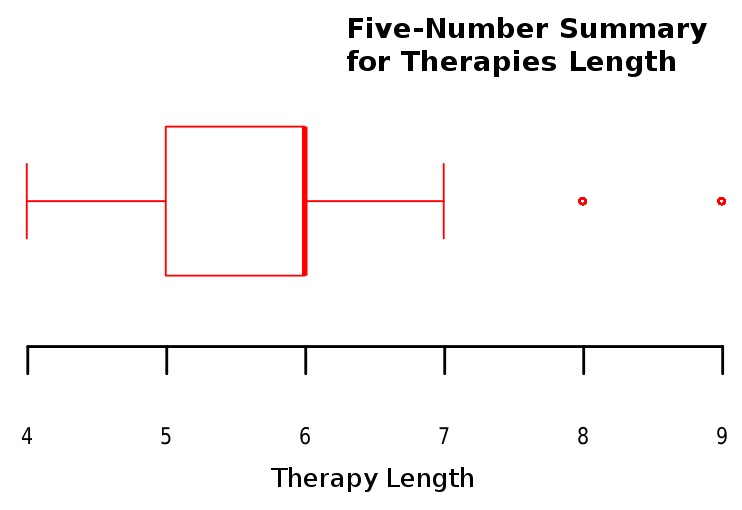
\includegraphics[width=\linewidth]{images/therapy_length.png}
  El gr\'afico revela que la mayor\'ia de las terapias tienen longitud 6 y otra gran cantidad tienen como longitud, 5. Con una menor frecuencia se
  encuentran las terapias con longitudes de 6 y 7, mientras que en muy pocos casos, las mismas alcanzaron valores de 8 o 9. La importancia de estas 
  estad\'isticas residen en el hecho de que mientras m\'as larga es la terapia, m\'as tiempo el paciente podr\'a ser mantenido bajo tratamiento, inhibiendo 
  as\'i el desarrollo de la enfermedad.

\subsection{Sobre la Energ\'ia Libre de las Mutaciones en Relaci\'on a la Longitud de Terapia}
  Cuando un antirretroviral es aplicado, la secuencia de nucle\'otidos que representa el ADN del virus sufre una modificaci\'on, es decir, se produce una
  secuencia mutante y su Energ\'ia libre var\'ia. La idea de este resumen estad\'istico es mostrar c\'omo la energ\'ia libre de las mutaciones se
  incrementa o decrementa acorde se avanza sobre la terapia.\\
  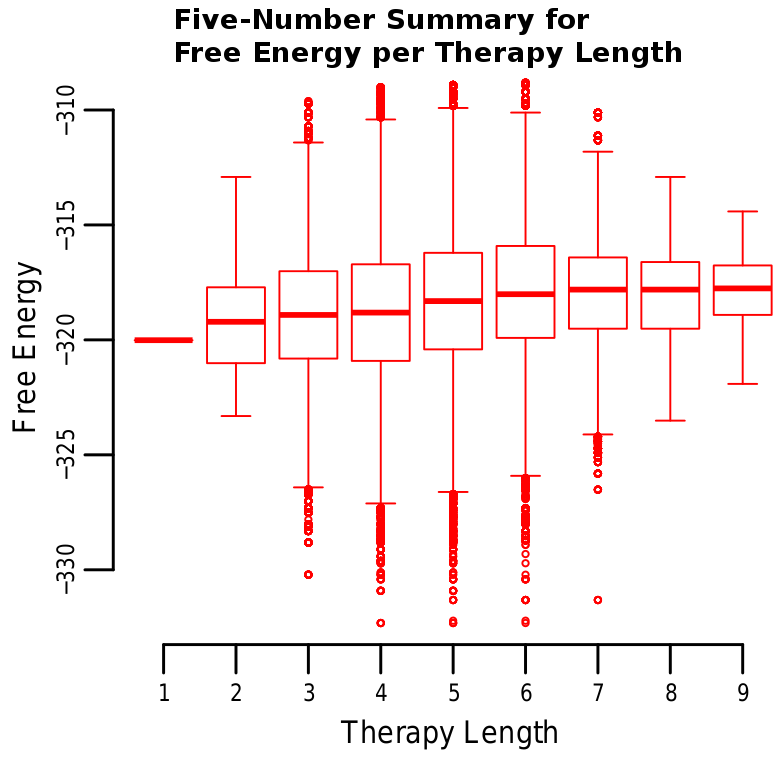
\includegraphics[width=\linewidth]{images/free_energy_by_thrapy_length.png}\\
  Tal y como se puede observar en el gr\'afico, a medida que se avanza en las terapias, los valores promedio para la energ\'ia libre se incrementan
  de manera moderada. Si bien estas variaciones son peque\~nas, las mismas informan que, en la mayor\'ia de los casos, a lo largo de un tratamiento
  el virus sufre cierta desestabilizaci\'on.

\subsection{Estimaci\'on de Tendencia de la Energ\'ia Libre}
  Los datos representados en el siguiente gr\'afico no var\'ian respecto del punto anterior, la \'unica diferencia es que se exhiben de otra manera.
  Esto se realiz\'o para obtener informaci\'on acerca de la tendencia\footnote{\url{www.en.wikipedia.org/wiki/Trend\_estimation}} de la energ\'ia libre a medida 
  que se van aplicando los antirretrovirales de la terapia.\\

  \begin{figure}[H]\hspace{-2cm}
    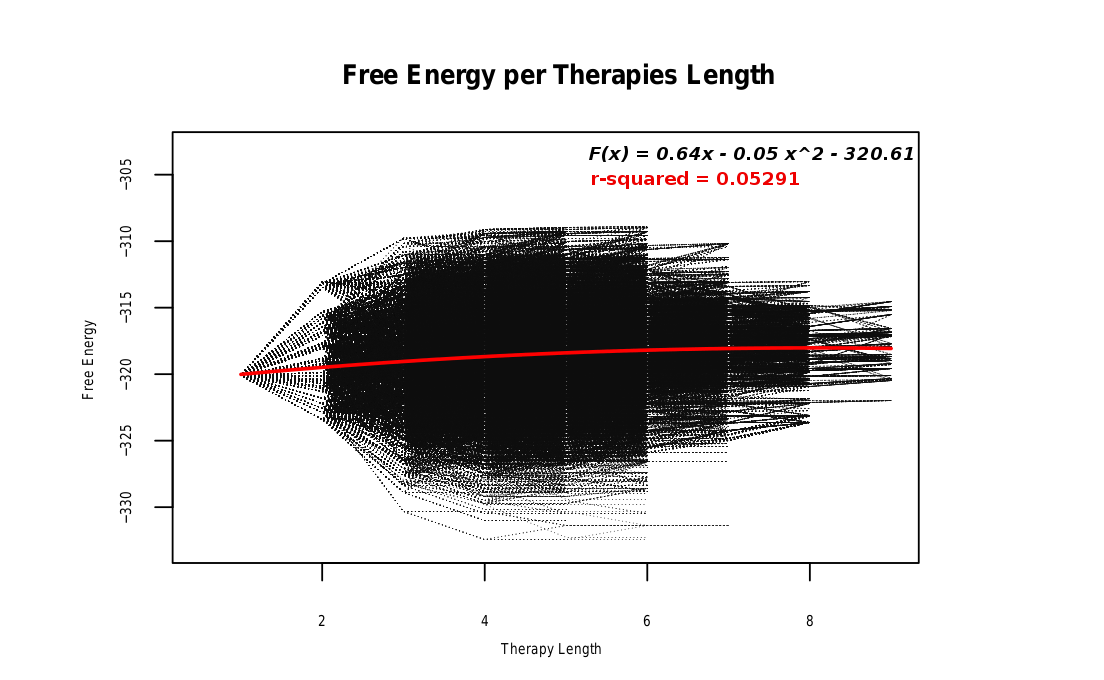
\includegraphics[scale=0.47]{images/ffe_vs_thLength.png}
  \end{figure}
    Como muestra el gr\'afico, los datos se encuentran de manera dispersa. La l\'inea roja que cruza el gr\'afico de nubes representa la tendencia. La
  f\'ormula de dicha l\'inea esta dada por la ecuaci\'on:\\ 
  \newline
  \emph{Y = 0.64X + -0.05$X^{2}$ - 320.61} \\ 
  \newline
  y su $R ^{2}$ es de 0.05291. Si bien el $R ^{2}$ es peque\~no, lo cual significa que
  la ecuaci\'on no aproxima con gran exactitud, se esperan obtener resultados m\'as precisos cuando la herramienta compute el \'arbol de ejecuci\'on
  de manera completa.
